\documentclass{article}

\usepackage{lipsum}
\usepackage[margin=1in,includefoot]{geometry}
\usepackage{graphicx}
\usepackage{float}
\usepackage[hidelinks]{hyperref}
\usepackage{amsmath}
\usepackage{lscape}

\usepackage[english]{babel}
\usepackage[utf8x]{inputenc}
\usepackage{multirow}
\usepackage{float}
\usepackage{multirow}
\usepackage[superscript,biblabel]{cite}




% Header and Footer Stuff
\usepackage{fancyhdr}
\pagestyle{fancy}
\fancyhead{}
\fancyfoot{}
\fancyfoot[R]{\thepage}
\renewcommand{\headrulewidth}{0pt}
\renewcommand{\footrulewidth}{0pt}

\begin{document}

\begin{titlepage}
	\begin{center}
	\line(1,0){300}\\
	[0.25in]
	\huge{\bfseries ST2004 Applied Probability}\\
	[2mm]
	\line(1,0){200}\\
	[1.5cm]
	\textsc{\LARGE ST2004 Individual Project }\\
	[0.75cm]
	\textsc{\Large Boxing Probability}\\
	[9cm]	
	\end{center}
	
	\begin{flushright}
	\textsc{\large Alexandru Sulea\\
	D Stream\\
	\#12315152\\
	27 October 2015\\}
	\end{flushright}

\end{titlepage}
%Table of Contents Stuff%
\tableofcontents
%\listoffigures
%\addcontentsline{toc}{section}{List of Figures}
\listoftables
\addcontentsline{toc}{section}{List of Tables}


\thispagestyle{empty}
\cleardoublepage
\pagenumbering{arabic}
\setcounter{page}{1}


\section{Introduction}\label{sec:intro}
The purpose of this project is to become more competent in probabilistic and statistical system and determination. It serves as an introduction to applying statistical probabilities in Excel and through large simulations determine the most probable outcome.\\
For this project, based on the research data on kangaroo behaviour, I chose to investigate if fights between humans could be predicted with the same certainty as a kangaroo fight. Or if perhaps there were other underlying factors which would have a significant impact on the data.


\section{Theory}\label{sec:theory}

\subsection{Kangaroo Combat }
In late 2004 a group of researchers found out that during a kangaroos migration season the males would engage in a form of ritualistic combat to determine dominance and rights to access to food and mates.\cite{one} \\
Upon closer observation the researchers noticed that while the combat was given consent by both parties participating the kangaroo who punched or kicked first, or seized the initiative would win a fight.\\
It was assessed if the kangaroo who initiated the contact first was older, thus having more experience against a younger opponent or if the initiating kangaroo was bigger thus having more confidence. Variables which might skew the finding, since therefore older and bigger males would almost always win over younger less experienced males due to size and experience. Or perhaps older males would win fights because their arms were longer and therefore better developed, thus able to reach a younger opponent before the reacting party.
The study found that older males, although challenged to fights by younger males would almost always deny the challenge.\cite{one}\\
Therefore in a fight between two kangaroos, both opponents are evenly matched, it seems that the more aggressive kangaroo will win.



\subsection{Human Combat }


I was curious to see if the same was true for human combat. Where two fighters enter a ring would the one who punched decisively first win the fight with the same probability as the kangaroos. If having more experience and age would be a factor or maybe it was arm reach which made the decisive between winners and losers.\\
Unfortunately match data on the UFC, which offers not only broad statistics on fighters but allows an entire array of fighting styles, was not publicly available. This was unfortunately unattainable due to the stringent copyright conditions enforced on footage of the fights by UFC.Short of torrenting 100Gb of fight videos the data was unattainable.\\

Upon further research a fight archive was found of decisive world renown boxing fights. These fights also showed the fighters age, reach and weight.\cite{five} All the important factors needed to calculate the data and quantify it in a table.\\
The videos were not watched in their entirety as some fights drag out to the full time allocated for the match. Instead the data was retrieved from the introduction at the start of the match, then the video would be fast forwarded to the first round.\cite{five} \\
There it was observed whichever party was more dominant during that match, with first physical contact noted down. The physical contact was not taken as contact of glove on glove, but rather glove on head or torso.\\



Due to the lack of available match data on UFC fights, there could not be a significant enough quantization of the that  data. The reason why UFC would be more realistic than boxing as a substitute for real life is the ability of MMA fighters to be able to kick and grasp their opponent. This is important, because, as a fight drags on, the fighters tend to grasp each other more, and seek a way to rest while inflicting more critical damage to their opponent.\\
Even though this is not as clear a stand-up boxing match, it's still important because a more experienced fighter will naturally be able to outmaneuver their opponent and win, even if they sustained more damage at the beginning of the match.\\
Thus the data for the following study was collected from a neatly organized play list of videos found on YouTube. The play list had a full fight video of every "sensational" boxing match from 1956 to 2013. The beginning of the video would also show the fighters physical stats, these were the stats that were also recorded.\\
Match history was not taken into account as every match was seen as an independent and mutually exclusive event.

 

\pagebreak
\section{Results}\label{sec:result}




\begin{table}[H]
\centering
\caption{1st Fighter Table}
\label{my-label}
\begin{tabular}{|l|l|l|l|l|}
\hline
No.   & \multicolumn{4}{l|}{Fighter1}          \\ \hline
0     & Name           & Age (years) & Height (cm) & Weight (kg) \\ \hline
1     & Ken Norton     &     &        & 100    \\ \hline
2     & Arturo Gatti   &     &        & 59     \\ \hline
3     & Gallo Estrada  & 22  & 170.18 & 49     \\ \hline
4 ... & James Toney    & 23  & 180.34 & 72     \\ \hline
50    & Vitai Klitchko & 38  & 200    & 144    \\ \hline
\end{tabular}
\end{table}
The following tables show how the data was recorded. The fighters name was important later on to detect which fighter group the winner came from and thus be able to compare stats to the respective looser.


\begin{table}[H]
\centering
\caption{2nd Fighter Table}
\label{my-label}
\begin{tabular}{|l|l|l|l|l|}
\hline
No.   & \multicolumn{4}{l|}{Fighter2}                                  \\ \hline
0     & Name                 & Age (years) & Height (cm) & Weight (kg) \\ \hline
1     & Larry Holmes         &             &             & 95          \\ \hline
2     & Wilson Rodriguez     &             &             & 58          \\ \hline
3     & Chocolatito Gonzalez & 25          & 160.02      & 49          \\ \hline
4 ... & Mike McCallum        & 35          & 180.34      & 71          \\ \hline
50    & Chris Diaz           & 28          & 181         & 113         \\ \hline
\end{tabular}
\end{table}
As can be seen there is some data missing from some fighters, this was an unfortunate side effect of old or corrupted video which was missing parts of the fighters stats, thus what little data is available was taken from the fight announcer.




\begin{table}[H]
\centering
\caption{Outcomes}
\label{my-label}
\begin{tabular}{|l|l|l|l|l|l|}
\hline
Fight & \multicolumn{5}{l|}{}                                                \\ \hline
0     & First Contact & Limb     & Winner               & Method & Outcome   \\ \hline
1     & ken Norton    & Left Arm & Larry Holmes         & TKO    & different \\ \hline
2     & Arturo Gatti  & Left Arm & Arturo Gatti         & KO     & same      \\ \hline
3     & Gallo Estrada & left Arm & Chocolatito Gonzalez & TKO    & different \\ \hline
4 ... & Mike McCallum & left Arm & James Toney          & TKO    & different \\ \hline
50     & Vitai Klitchko   & Right Arm & Vitai Klitchko         & KO     & different \\ \hline
\end{tabular}
\end{table}

\begin{figure}[H]
\centering
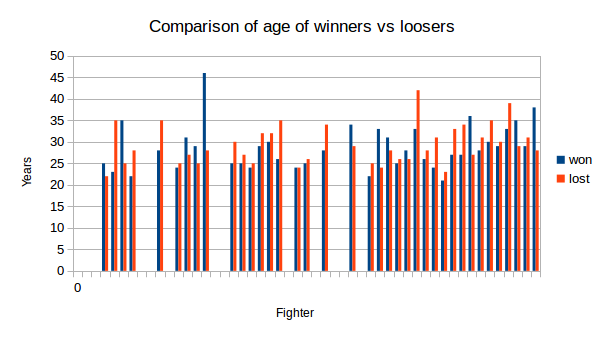
\includegraphics[width=0.5\textwidth]{a10.png}

\end{figure}

\begin{align*}
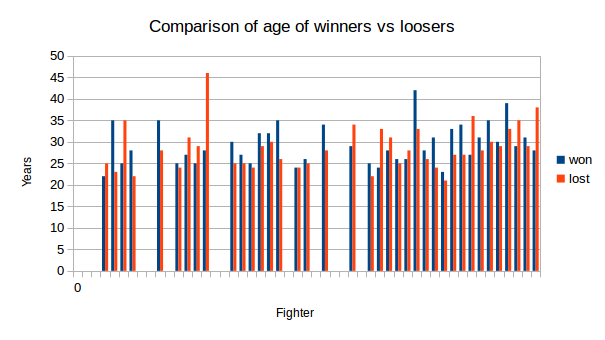
\includegraphics[height=1.8in]{a4.png}
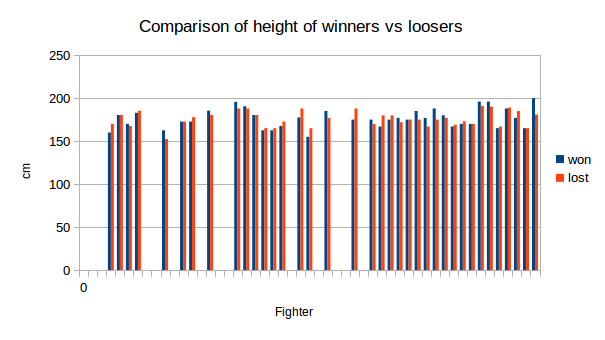
\includegraphics[height=1.8in]{a5.png}
\end{align*}\\

As can be seen in the above graph, the winner and losers stats have been placed side by side for a better graphical representation to show how much: older, taller, heavier the winners were from the losers. 

\begin{table}[H]
\centering
\caption{Averages}
\label{my-label}
\begin{tabular}{|l|l|l|l|}
\hline
Average & Age  & Height & Weight \\ \hline
Winner  & 28.6 & 72.4   & 176.5  \\ \hline
Looser  & 29.3 & 71.5   & 176.1  \\ \hline
Overall & 29.0 & 72.0   & 176.3  \\ \hline
\end{tabular}
\end{table}
The table of averages takes the statistics from the winners and losers to show an average and through this average show a pattern of the ideal age to be a fighter and the predominately loosing age of a fighter. The two are very close together, with a difference of 9 months between a loosing and winning fighters age. Through the results obtained though it is clear that a fighter becomes less effective after passing the age of 30.\\
The statistics also show that winners had a slight height and weight advantage over the losers. This possibly enabled the winning fighters to hit harder while out of reach of their opponents.




\begin{figure}[H]
\centering
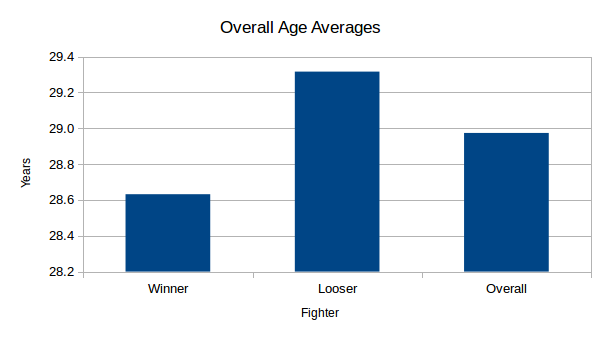
\includegraphics[width=0.5\textwidth]{a1.png}
\caption{Probability of Winning with Unbiased odds}
\end{figure}

\begin{align*}
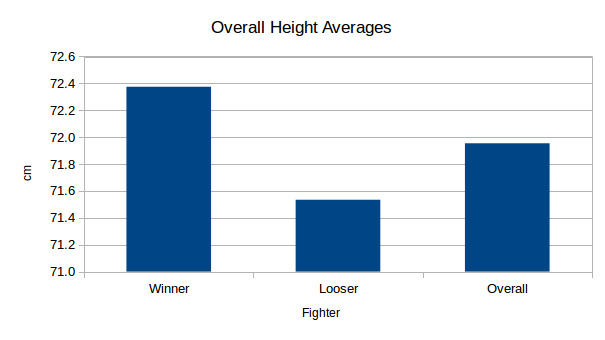
\includegraphics[height=1.8in]{a2.png}
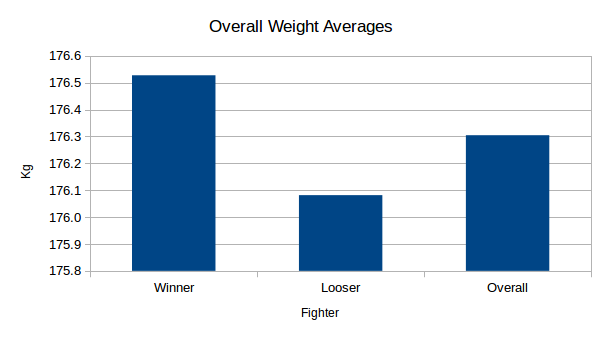
\includegraphics[height=1.8in]{a3.png}
\end{align*}\\


\begin{table}[H]
\centering
\caption{Frequency of winning and loosing}
\label{my-label}
\begin{tabular}{|l|l|}
\hline
Outcome & No. \\ \hline
win     & 21  \\ \hline
loose   & 29  \\ \hline
\end{tabular}
\end{table}

\begin{figure}[H]
\centering
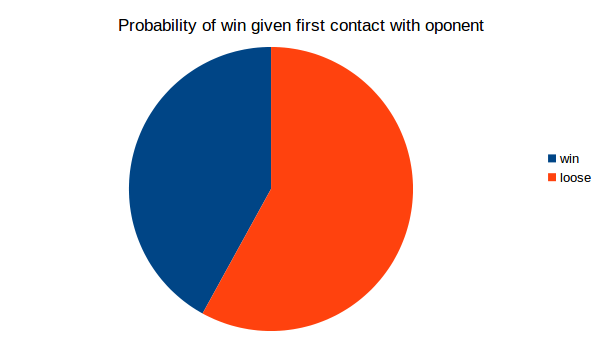
\includegraphics[width=0.5\textwidth]{a7.png}

\end{figure}

\begin{table}[H]
\centering
\caption{Frequency of first hit with respect to limbs}
\label{my-label}
\begin{tabular}{|l|l|}
\hline
LIMB      & No. \\ \hline
Left Arm  & 25  \\ \hline
Right Arm & 25  \\ \hline
\end{tabular}
\end{table}



\begin{table}[H]
\centering
\caption{Frequency of match endings with respect to knockouts and technical knockouts}
\label{my-label}
\begin{tabular}{|l|l|}
\hline
End & No. \\ \hline
KO  & 28  \\ \hline
TKO & 22  \\ \hline
\end{tabular}
\end{table}

\begin{align*}
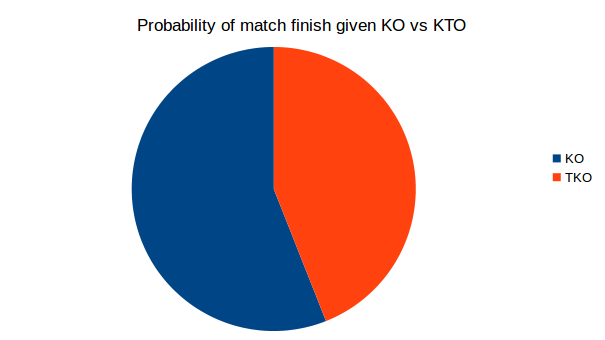
\includegraphics[height=1.8in]{a8.png}
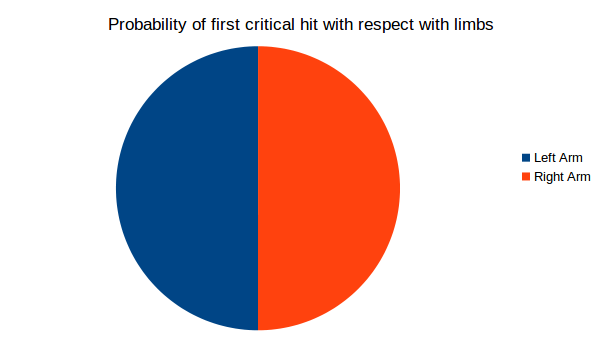
\includegraphics[height=1.8in]{a9.png}
\end{align*}\\

The following graphs and tables show the frequency of knockouts and TKO's. For this study I defined a KO as the opponent being knocked to the ground or disqualified and the TKO as a scorecard decision. 
The same vs. different category is a frequency of a fighter winning given that they were the more aggressive opponent. As can be observed from the table, no clear advantage is shown. Same for a predominant are used. The only clear distinctions discovered were age height and weight.


\pagebreak


\section{Discussion}\label{sec:discuss}

The preliminary results obtained show that a fight between consenting parties of similar age and experience is not won based on a fighters aggression. The engaging fighter, although dominant in the first minutes of the round tends to tire during the second or recurring rounds. This may also be a factor of the sport, in boxing , the fighters are required to wear heavily padded gloves and shorts with a high waistband. This does not eliminate the risk of injury but it does reduce it. Perhaps in a real life fistfight, the first dominant fighter would win most of the time as they can do more damage sooner to the reactive fighter.\cite{three} Facial cuts, fractured jaws and eye-sockets are common in street brawls. If one fighter can break their opponent's jaw or eye-socket they have thus rendered that opponent inactive for quite some time.\cite{four} The high waistbands in boxing also minimize damage to the torso and rib cage area. This again is not a reality in street fights where a fallen opponent can expect to be kicked in the head or the rib cage while on the ground.\\

The second observation made during this research project is the pre-fight activity the fighters engage in. Either during the pre-fight interviews or during the weigh-ins. The psychological games initiated by the fighters seem to make the other party more angry and therefore lose concentration. Fighting is a physical activity though, with fighters training years to achieve lightning reflexes and muscle memory thus an angry fighter would still make for a challenging adversary irrelevant of mind state. \\
Perhaps the reason fighters try to act dominant in the pre-fight appearances is not to intimidate their opponent but to make the opponent want to overcompensate for possibly a lackluster performance during the pre-fight events.\cite{2}\\
A fighter that is trying to overcompensate and seem dominant would be far more enticed to over reach and outperform their opponent, especially in the first round. Due to the padding and protection required in boxing the damage to the opponent would endure would be minimal.\cite{two} \\
At this point the second and less talked about part of fighting comes in. Kung Fu movies aside, a human being can only fight for a limited amount of time before becoming exhausted, even if one had an infinite amount of skill, through over exertion, they would still lose at some point.\\
Unlike running or swimming, fighting activates a different part of the human  brain. When a human being is fighting, even in an organized and sanctioned sport the flight or fight senses still activate.\cite{three}
This leads to a uniquely high  secretion of adrenaline, testosterone, ACTH and dopamine.\\
In layman's terms the body has sensed that it is in mortal danger, thus it will shut down all secondary and tertiary organs to limit injury or blood loss while increasing the blood flow and oxygen saturation in the circulatory system.The dopamine will also suppress the pain receptors while giving a feeling of light euphoria, suppressing fear.\cite{six}\\
Thus the body is now capable of performing at peak efficiency.\cite{seven} The problem lies in the very systems that help us achieve this super human strength is that since it was the secondary organs which secreted these substances, and those organs are now switched off, there is no constant flow through the body. \\
The fight or flight response is thus more of an instant boost than a reliable tap. \\
By going into this state, the body is also burning far more energy than it normally would leading to quicker exhaustion. 
Thus the fighter who can suppress their fight or flight urges and take a beating from a dominating opponent for long enough for the opponent to become exhausted wins almost every time. \\
Due to different measuring standards of arm reach between the different boxing organizations, that metric was not at all quantifiable, but it may have shown  that a fighter with longer arms to have a clear advantage over his opponent.\\




\pagebreak

\section{Conclusion}
	Due to the preliminary results obtained the conclusion drawn would be that there is very little to no advantage from either opponent attacking first. This is most probably a bi-product of years of training and conditioning in physical combat.
Thus we can say definitively that the strategy of "getting inside your opponents head" is ineffective, at least against a skilled opponent.\\
Overall the study has shown that the ideal age when a fighter seems to be at their peak is 28, and that a weight advantage does matter. Sometimes 1kg can be the difference between winning and loosing.
	
	
	


\appendix


	
	\begin{thebibliography}{3}
  %league
  \bibitem{one}
  \emph{Kangaroos: Biology of the Largest Marsupials}, Dawson, Terence J, (1995).  Cornell University Press/Comstock Publishing.
  
  \bibitem{two}

  \emph{Stress Management for Health Course. "The Fight Flight Response"},
 

  \bibitem{four}

  \emph{The Science of Stress },Olpin, Michael, 
  Weber State University.
  
  \bibitem{three}

  \emph{What's the purpose of the fight or flight response? },Grohol, John, 
  18 April 2013.


   \bibitem{five}
  \emph{https://www.youtube.com/playlist?list=PLQcJnkxSzA8ypDBwz9wbP87MN4dNwklBO},

 \bibitem{six}
  \emph{ACTH Action on the Adrenal },Margioris, Andrew, Tsatsanis, Christos
   April 2011
   

  
  \bibitem{seven}
  \emph{Autonomic Nervous System }, Schmidt, A; Thews, G (1989)
   pp. 333–370
\end{thebibliography}


\end{document}